\chapter{重积分}
\section{二重积分}
\subsection{二重积分的概念}
\begin{definition}
设\(f(x,y)\)是有界闭区域\(D\)上的有界函数.将闭区域\(D\)任意分成\(n\)个小闭区域\[
\increment\sigma_1,\increment\sigma_2,\dotsc,\increment\sigma_n,
\]其中\(\increment\sigma_i\)表示第\(i\)个小闭区域,%
也表示它的面积.
在每个\(\increment\sigma_i\)上任取一点\(\opair{\xi_i,\eta_i}\),%
作乘积\(f(\xi_i,\eta_i) \increment\sigma_i\)(\(i=1,2,\dotsc,n\)),%
并作和\(\sum\limits_{i=1}^n f(\xi_i,\eta_i) \increment\sigma_i\).
如果当各小闭区域的直径中的最大值\(\lambda\)趋于零时,%
这和的极限总存在,%
则称此极限为“函数\(f(x,y)\)在闭区域\(D\)上的\DefineConcept{二重积分}(double integral)”,%
记作\(\iint_D f(x,y) \dd{\sigma}\),即
\begin{gather}
\iint_D f(x,y) \dd{\sigma}
= \lim\limits_{\lambda\to0} \sum\limits_{i=1}^n f(\xi_i,\eta_i) \increment\sigma_i,
\tag1
\end{gather}
其中\(f(x,y)\)叫做\DefineConcept{被积函数},%
\(f(x,y) \dd{\sigma}\)叫做\DefineConcept{被积表达式},%
\(\dd{\sigma}\)叫做\DefineConcept{面积元素},%
\(x\)与\(y\)叫做\DefineConcept{积分变量},%
\(D\)叫做\DefineConcept{积分区域},%
\(\sum\limits_{i=1}^n f(\xi_i,\eta_i) \increment\sigma_i\)叫做\DefineConcept{积分和}.

如果函数\(f(x,y)\)在闭区域\(D\)上的二重积分存在,那么就说\(f(x,y)\)在\(D\)上\DefineConcept{可积},%
记作\(f \in R(D)\).

在二重积分的定义中对闭区域\(D\)的划分是任意的.
如果在直角坐标系中用平行于坐标轴的直线网来划分\(D\),%
那么面积元素\(\dd{\sigma}\)可以改为记作\(\dd{x}\dd{y}\),进而把二重积分记作\[
\iint_{D}{f(x,y)\dd{x}\dd{y}},
\]其中\(\dd{x}\dd{y}\)叫做\DefineConcept{直角坐标系中的面积元素}.
\end{definition}

\begin{theorem}[充分条件]
设函数\(f(x,y)\)在闭区域\(D\)上连续,则\(f(x,y)\)在\(D\)上可积.
\end{theorem}

\subsection{二重积分的几何性质}
一般的,如果\(f(x,y) \geqslant 0\),被积函数\(f(x,y)\)可解释为曲顶柱体的顶在点\(\opair{x,y}\)处的竖坐标,所以二重积分的几何意义就是柱体的体积.如果\(f(x,y) < 0\),柱体就在\(xOy\)面的下方,二重积分的绝对值仍等于柱体的体积,但二重积分的值是负的.如果\(f(x,y)\)在\(D\)的部分区域上是正的,而在其他的部分区域上是负的,那么\(f(x,y)\)在\(D\)上的二重积分就等于\(xOy\)面上方的柱体体积减去\(xOy\)面下方的柱体体积所得之差.

\subsection{二重积分的性质}
\begin{property}\label{theorem:重积分.二重积分的性质1}
设\(\alpha\)、\(\beta\)为常数,则\[
\iint_D [\alpha f(x,y)+\beta g(x,y)] \dd{\sigma}
=\alpha \iint_D f(x,y) \dd{\sigma}
+\beta \iint_D g(x,y) \dd{\sigma}.
\]
\end{property}

\begin{property}\label{theorem:重积分.二重积分的性质2}
如果闭区域\(D\)被有限条曲线分为有限个部分闭区域,则在\(D\)上的二重积分等于在各部分闭区域上二重积分的和,即\[
D = \bigcup_{i=1}^n D_i
\implies
\iint_D f(x,y) \dd{\sigma}
= \sum\limits_{i=1}^n \iint_{D_i} f(x,y) \dd{\sigma}.
\]
\end{property}
这个性质表示二重积分对于积分区域具有\DefineConcept{可加性}.

\begin{property}\label{theorem:重积分.二重积分的性质3}
如果在\(D\)上,\(f(x,y)=1\),\(\sigma\)为\(D\)的面积,则\[
\iint_D 1\cdot\dd{\sigma}
=\iint_D \dd{\sigma}
=\sigma.
\]
\end{property}

\begin{property}\label{theorem:重积分.二重积分的性质4}
如果在\(D\)上,\(f(x,y) \leqslant \varphi(x,y)\),则有\[
\iint_D f(x,y) \dd{\sigma} \leqslant \iint_D \varphi(x,y) \dd{\sigma}.
\]

特别地,\[
\abs{\iint_D f(x,y) \dd{\sigma}} \leqslant \iint_D \abs{f(x,y)} \dd{\sigma}.
\]
\end{property}

\begin{property}\label{theorem:重积分.二重积分的性质5}
设\(M\)、\(m\)分别是\(f(x,y)\)在闭区域\(D\)上的最大值和最小值,\(\sigma\)是\(D\)的面积,则有\[
m\sigma \leqslant \iint_D f(x,y) \dd{\sigma} \leqslant M\sigma.
\]
\end{property}
上述不等式对于二重积分估值的不等式.

\begin{property}[二重积分的中值定理]\label{theorem:重积分.二重积分的中值定理}
设函数\(f(x,y)\)在闭区域\(D\)上连续,\(\sigma\)是\(D\)的面积,则在\(D\)上至少存在一点\(\opair{\xi,\eta}\),使得\[
\iint_D f(x,y) \dd{\sigma} = \sigma \cdot f(\xi,\eta).
\]
\begin{proof}
显然\(\sigma\neq0\).把\cref{theorem:重积分.二重积分的性质5} 中的不等式各除以\(\sigma\),有\[
m
\leqslant
\zeta = \frac{1}{\sigma} \iint_D f(x,y) \dd{\sigma}
\leqslant
M.
\]
这就是说,确定的数值\(\zeta\)是%
介于函数\(f(x,y)\)的最大值\(M\)与最小值\(m\)之间的.
根据\cref{theorem:多元函数微分法.介值定理},%
在\(D\)上存在一点\(\opair{\xi,\eta}\)%
使得函数在该点的值\(f(\xi,\eta)\)%
与上述的确定的数值\(\zeta\)相等,即\[
f(\xi,\eta) = \zeta,
\]上式两端各乘以\(\sigma\),记得所要证明的公式.
\end{proof}
\end{property}

\begin{example}
设\(f(x,y) = f_1(x) \cdot f_2(y)\),证明:\[
\iint_D f(x,y) \dd{x} \dd{y}
= \left[ \int_a^b f_1(x) \dd{x} \right] \cdot \left[ \int_c^d f_2(y) \dd{y} \right],
\]其中\(D = \Set{\opair{x,y} \given a \leqslant x \leqslant b, c \leqslant y \leqslant d}\).
\end{example}

\subsection{二重积分的计算法}
直接按照二重积分的定义来计算二重积分,对少数特别简单的被积函数和积分区域来说是可行的.但对一般的函数和区域来说,这不是一种切实可行的方法.这里介绍一种计算二重积分的方法,即把二重积分化为两次单积分(即两次定积分)来计算.

\subsubsection{利用直角坐标系计算二重积分}
\begin{theorem}[X型区域]
设积分区域\(D\)可以用不等式\begin{gather*}
a \leqslant x \leqslant b, \\
\varphi_1(x) \leqslant y \leqslant \varphi_2(x),
\end{gather*}来表示,其中函数\(\varphi_1(x)\)、\(\varphi_2(x)\)在区间\([a,b]\)上连续,那么有\[
\iint_D f(x,y) \dd{\sigma}
=\int_a^b \dd{x} \int_{\varphi_1(x)}^{\varphi_2(x)} f(x,y) \dd{y}.
\]
\end{theorem}
X型区域\(D\)的特点是:
任一穿过\(D\)内部且平行于\(y\)轴的直线与\(D\)的边界相交不多于两点.

\begin{theorem}[Y型区域]
设积分区域\(D\)可以用不等式\begin{gather*}
\psi_1(y) \leqslant x \leqslant \psi_2(y), \\
c \leqslant y \leqslant d,
\end{gather*}来表示,其中函数\(\psi_1(x)\)、\(\psi_2(x)\)在区间\([c,d]\)上连续,那么就有\[
\iint_D f(x,y) \dd{\sigma}
=\int_c^d \dd{y} \int_{\psi_1(x)}^{\psi_2(x)} f(x,y) \dd{x}.
\]
\end{theorem}
Y型区域\(D\)的特点是:
任一穿过\(D\)内部且平行于\(x\)轴的直线与\(D\)的边界相交不多于两点.

\begin{corollary}
如果积分区域\(D\)既是X型的,又是Y型的,则有\[
\int_a^b \dd{x}
 \int_{\varphi_1(x)}^{\varphi_2(x)} f(x,y) \dd{y}
=\int_c^d \dd{y}
 \int_{\psi_1(x)}^{\psi_2(x)} f(x,y) \dd{x}.
\]

但是,在化二重积分为二次积分时,为了计算简便,需要选择恰当的二次积分的顺序.
这时,既要考虑积分区域\(D\)的形状,又要考虑被积函数\(f(x,y)\)的特性.
\end{corollary}

\subsubsection{利用极坐标计算二重积分}
有些二重积分,积分区域\(D\)的边界曲线用极坐标方程来表示比较方便,且被积函数用极坐标变量\(\rho\)、\(\theta\)表达比较简单.这时,就可以考虑利用极坐标来计算二重积分.

下面我们按二重积分的定义\[
\iint_D f(x,y) \dd{\sigma}
= \lim\limits_{\lambda\to0} \sum\limits_{i=1}^n f(\xi_i,\eta_i) \increment\sigma_i
\]来研究一下这个和的极限在极坐标系中的形式.

假定从极点\(O\)出发且穿过闭区域\(D\)内部的射线与\(D\)的边界曲线相交不多于两点.
我们用以极点为中心的一族同心圆\(\rho = \text{常数}\),%
以及从极点出发的一族射线\(\theta = \text{常数}\),%
把\(D\)划分为\(n\)个小闭区域.
除了包含边界点的一些小闭区域外,其他小闭区域的面积\(\increment\sigma_i\)可计算如下:
\begin{align*}
\increment\sigma_i
&= \frac{1}{2} (\rho_i+\increment\rho_i)^2 \cdot \increment\theta_i
- \frac{1}{2} \rho_i^2 \cdot \increment\theta_i \\
&= \frac{1}{2} (2\rho_i + \increment\rho_i) \increment\rho_i \cdot \increment\theta_i \\
&= \frac{\rho_i + (\rho_i+\increment\rho_i)}{2} \cdot \increment\rho_i \cdot \increment\theta_i \\
&= \overline{\rho}_i \cdot \increment\rho_i \cdot \increment\theta_i,
\end{align*}
其中\(\overline{\rho}_i\)表示相邻两端圆弧的半径的平均值.
在这小闭区域内取圆周\(\rho = \overline{\rho}_i\)上的一点\(\opair{\overline{\rho}_i,\overline{\theta}_i}\),该点的直角坐标设为\(\opair{\xi_i,\eta_i}\),则由直角坐标系与极坐标系之间的关系有\(\xi_i = \overline{\rho}_i \cos\overline{\theta}_i,
\eta_i = \overline{\rho}_i \sin\overline{\theta}_i\).
于是\[
\lim\limits_{\lambda\to0} \sum\limits_{i=1}^n f(\xi_i,\eta_i) \increment\sigma_i
= \lim\limits_{\lambda\to0} \sum\limits_{i=1}^n f(\overline{\rho}_i \cos\overline{\theta}_i,\overline{\rho}_i \sin\overline{\theta}_i) \overline{\rho}_i \cdot \increment\rho_i \cdot \increment\theta_i,
\]即\[
\iint_D f(x,y) \dd{\sigma}
= \iint_D f(\rho\cos\theta,\rho\sin\theta) \rho \dd{\rho} \dd{\theta}.
\]

这里我们把点\(\opair{\rho,\theta}\)看作在同一平面上的点\(\opair{x,y}\)的极坐标表示,所以上式右端的积分区域仍然记作\(D\).

由于在直角坐标系中\(\iint_D f(x,y) \dd{\sigma}\)也常记作\(\iint_D f(x,y) \dd{x} \dd{y}\),所以上式又可以写成
\begin{equation}\label{equation:线性方程组.二重积分坐标变换公式}
\iint_D f(x,y) \dd{x} \dd{y}
= \iint_D f(\rho\cos\theta,\rho\sin\theta) \rho \dd{\rho} \dd{\theta},
\end{equation}
这就是二重积分的变量从直角坐标变换为极坐标的变换公式,%
其中\(\rho \dd{\rho} \dd{\theta}\)就是极坐标系中的面积元素.

\cref{equation:线性方程组.二重积分坐标变换公式} 表明,%
要把二重积分中的变量从直角坐标变换为极坐标,%
只要把被积函数中的\(x\)、\(y\)分别换成\(\rho \cos\theta\)、\(\rho \sin\theta\),%
并把直角坐标系中的面积元素\(\dd{x} \dd{y}\)换成极坐标系中的面积元素\(\rho \dd{\rho} \dd{\theta}\).

极坐标系中的二重积分,同样可以化为二次积分来计算.
\begin{theorem}
设积分区域可以用不等式\begin{gather*}
0 \leqslant \varphi_1(\theta) \leqslant \rho \leqslant \varphi_2(\theta), \\
0 \leqslant \alpha \leqslant \theta \leqslant \beta \leqslant 2\pi,
\end{gather*}来表示,其中函数\(\varphi_1(\theta)\)、\(\varphi_2(\theta)\)在区间\([\alpha,\beta]\)上连续,那么利用以下关系\[
\left\{ \begin{array}{l}
x = \rho\cos\theta \\
y = \rho\sin\theta \\
\end{array} \right.
\quad\text{或}\quad
\left\{ \begin{array}{l}
\rho = \sqrt{x^2+y^2} \\
\tan\theta = y/x \quad (x \neq 0) \\
\end{array} \right.,
\]替换二重积分\(\iint_{D}{f(x,y)\dd{x}\dd{y}}\)中的积分变量,即有
\begin{equation}
\iint_D f(\rho\cos\theta,\rho\sin\theta) \rho \dd{\rho} \dd{\theta}
=\int_{\alpha}^{\beta} \left[
	\int_{\varphi_1(\theta)}^{\varphi_2(\theta)}
		f(\rho\cos\theta,\rho\sin\theta) \rho \dd{\rho} \right] \dd{\theta}.
\end{equation}
上式也可写作
\begin{equation}
\iint_D f(\rho\cos\theta,\rho\sin\theta) \rho \dd{\rho} \dd{\theta}
=\int_{\alpha}^{\beta} \dd{\theta}
	\int_{\varphi_1(\theta)}^{\varphi_2(\theta)}
		f(\rho\cos\theta,\rho\sin\theta) \rho \dd{\rho}.
\end{equation}
\end{theorem}

\begin{corollary}
设区域\(D\)在极坐标系中是由射线\(\theta=\alpha\)、\(\theta=\beta\)和曲线\(\rho=\varphi_1(\theta)\)、\(\rho=\varphi_2(\theta)\)围成的,则区域\(D\)的面积为
\begin{equation}
\sigma = \iint_D \rho \dd{\rho} \dd{\theta}
= \frac{1}{2} \int_{\alpha}^{\beta} [\varphi_2^2(\theta) - \varphi_1^2(\theta)] \dd{\theta}.
\end{equation}

特别地,如果区域\(D\)在极坐标系中是由射线\(\theta=\alpha\)、\(\theta=\beta\)和曲线\(\rho=\varphi(\theta)\)围成的曲边三角形,则这个曲边三角形的面积为
\begin{equation}
\sigma = \frac{1}{2} \int_{\alpha}^{\beta} \varphi^2(\theta) \dd{\theta}.
\end{equation}
\end{corollary}

\begin{example}
证明:半径为\(r\)的圆内的面积为\(S = \pi r^2\).
\begin{proof}
以圆心为原点建立极坐标系,得圆内的方程为\[
D: \rho \leqslant r.
\]那么圆内的面积为\[
S = \iint_D \rho \dd{\rho} \dd{\theta}
= \int_0^{2\pi} \dd{\theta} \int_0^r \rho \dd{\rho}
= 2\pi \cdot \frac{1}{2} r^2
= \pi r^2.
\qedhere
\]
\end{proof}
\end{example}

\begin{example}
计算\(\iint_D e^{-x^2-y^2} \dd{x} \dd{y}\),其中\(D\)是由中心在原点、半径为\(a\)的圆周所围成的闭区域.
\begin{solution}
在极坐标系中,闭区域\(D\)可以表示为\begin{gather*}
0 \leqslant \rho \leqslant a, \\
0 \leqslant \theta \leqslant 2\pi,
\end{gather*}那么有\[
\iint_D e^{-x^2-y^2} \dd{x} \dd{y}
= \iint_D e^{-\rho^2} \rho \dd{\rho} \dd{\theta}
= \int_0^{2\pi} \dd{\theta} \int_0^a e^{-\rho^2} \rho \dd{\rho}
= \pi(1-e^{-a^2}).
\]
\end{solution}
\end{example}

利用上面的结论,可以计算常用的反常积分\(\int_0^{+\infty} e^{-x^2} \dd{x}\).
\begin{example}
求\(\int_0^{+\infty} e^{-x^2} \dd{x}\).
\begin{solution}
设\begin{align*}
D_1 &= \{ \opair{x,y} \mid x^2+y^2 \leqslant R^2 \land x \geqslant 0 \land y \geqslant 0 \}, \\
D_2 &= \{ \opair{x,y} \mid x^2+y^2 \leqslant 2 R^2 \land x \geqslant 0 \land y \geqslant 0 \}, \\
S &= \{ \opair{x,y} \mid 0 \leqslant x \leqslant R \land 0 \leqslant y \leqslant R \}.
\end{align*}显然\(D_1 \subseteq S \subseteq D_2\).
由于\(e^{-x^2-y^2} > 0\),从而在这些闭区域上的二重积分之间有有不等式\[
\iint_{D_1} e^{-x^2-y^2}\dd{x}\dd{y}
< \iint_{S} e^{-x^2-y^2}\dd{x}\dd{y}
< \iint_{D_2} e^{-x^2-y^2}\dd{x}\dd{y}.
\]因为\[
\iint_{S}{e^{-x^2-y^2}\dd{x}\dd{y}}
= \int_0^R e^{-x^2}\dd{x} \cdot \int_0^R e^{-y^2} \dd{y}
= \left( \int_0^R e^{-x^2} \dd{x} \right)^2,
\]又有\begin{align*}
\iint_{D_1}{e^{-x^2-y^2}\dd{x}\dd{y}}
&= \frac{\pi}{4} (1 - e^{-R^2}) \\
\iint_{D_2}{e^{-x^2-y^2}\dd{x}\dd{y}}
&= \frac{\pi}{4} (1 - e^{-2 R^2})
\end{align*}于是上面的不等式可写成\[
\frac{\pi}{4} (1 - e^{-R^2})
< \left( \int_0^R e^{-x^2} \dd{x} \right)^2
< \frac{\pi}{4} (1 - e^{-2 R^2}).
\]令\(R \to +\infty\),上式两端均趋于同一极限\(\frac{\pi}{4}\),从而
\begin{equation}\label{equation:重积分.常用积分1}
\int_0^{+\infty} e^{-x^2} \dd{x} = \frac{\sqrt{\pi}}{2}.
\end{equation}
\end{solution}
\end{example}
对积分 \labelcref{equation:重积分.常用积分1} 稍作修改,可以得到误差函数\(\erf(z)\)的定义:
\begin{equation}
\erf(z) = \frac{2}{\sqrt{\pi}} \int_0^z e^{-t^2} \dd{t}.
\end{equation}

因为积分 \labelcref{equation:重积分.常用积分1} 的被积函数在\((-\infty,+\infty)\)上是偶函数,所以\begin{equation}\label{equation:重积分.常用积分2}
\int_{-\infty}^{+\infty} e^{-x^2} \dd{x} = \sqrt{\pi}.
\end{equation}

\subsubsection{二重积分被积函数的对称性}
\begingroup
\def\intx#1{\iint_{#1} f(x,y) \dd{\sigma}}
若\(D\)关于\(y\)轴对称,则\[
\intx{D} = \left\{ \begin{array}{cc}
2 \intx{D_1}, & f(x,y) = f(-x,y), \\
0, & f(x,y) = -f(-x,y),
\end{array} \right.
\]其中\(D_1\)是\(D\)在\(y\)轴左侧或右侧的部分.

若\(D\)关于\(x\)轴对称,则\[
\intx{D} = \left\{ \begin{array}{cc}
2 \intx{D_1}, & f(x,y) = f(x,-y), \\
0, & f(x,y) = -f(x,-y),
\end{array} \right.
\]其中\(D_1\)是\(D\)在\(x\)轴上侧或下侧的部分.

若\(D\)关于原点对称,则\[
\intx{D} = \left\{ \begin{array}{cc}
2 \intx{D_1}, & f(x,y) = f(-x,-y), \\
0, & f(x,y) = -f(-x,-y),
\end{array} \right.
\]其中\(D_1\)是\(D\)关于原点对称的半个部分.

若\(D\)关于\(y=x\)对称,则\[
\intx{D} = \left\{ \begin{array}{cc}
2 \intx{D_1}, & f(x,y) = f(y,x), \\
0, & f(x,y) = -f(y,x),
\end{array} \right.
\]其中\(D_1\)是\(D\)关于\(y=x\)对称的半个部分.

若\(D\)关于\(y=a\ (\neq0)\)对称,则\[
\intx{D} = \left\{ \begin{array}{cc}
2 \intx{D_1}, & f(x,y) = f(x,2a-y), \\
0, & f(x,y) = -f(x,2a-y),
\end{array} \right.
\]其中\(D_1\)是\(D\)在\(y=a\)上侧或下侧的部分.

若\(D\)关于\(x=a\ (\neq0)\)对称,则\[
\intx{D} = \left\{ \begin{array}{cc}
2 \intx{D_1}, & f(x,y) = f(2a-x,y), \\
0, & f(x,y) = -f(2a-x,y),
\end{array} \right.
\]其中\(D_1\)是\(D\)在\(x=a\)左侧或右侧的部分.

\def\op{\underset{(>)}{=}}
若将\(D\)中的\(x,y\)对换后,\(D\)不变,则有\[
\iint_D f(x,y) \dd{x}\dd{y} = \iint_D f(y,x) \dd{x}\dd{y} = I.
\]若进一步有\(f(x,y)+f(y,x) \op a\),则\[
I = \frac{1}{2} \iint_D [ f(x,y) + f(y,x) ] \dd{x}\dd{y}
\op \frac{1}{2} \iint_D a \dd{x}\dd{y}
= \frac{a}{2} S_D,
\]其中,\(S_D\)是\(D\)的面积.
\endgroup

\subsubsection{二重积分的换元法}
\begin{theorem}
设二元函数\(f(x,y)\)在\(xOy\)平面上的闭区域\(D\)上连续,变换\[
T :\: \left\{ \begin{array}{l}
x = x(u,v), \\
y = y(u,v), \\
\end{array} \right.
\]将\(uOv\)平面上的闭区域\(G\)变为\(xOy\)平面上的\(D\),且满足:
\begin{enumerate}
\item \(x(u,v)\)、\(y(u,v)\)在\(G\)上具有一阶连续偏导数;
\item 在\(G\)上雅克比式\(J = \jacobi{x,y}{u,v} \neq 0\);
\item 变换\(T :\: G \to D\)是一一映射,%
\end{enumerate}
则有\begin{equation}\label{equation:重积分.二重积分的换元公式}
\iint_D f(x,y) \dd{x} \dd{y}
=\iint_G f[x(u,v),y(u,v)] \cdot \abs{J} \dd{u} \dd{v}.
\end{equation}
%证明@see: 《高等数学(第六版 下册)》P149
\end{theorem}
\cref{equation:重积分.二重积分的换元公式} 称为\DefineConcept{二重积分的换元公式}.
这里我们指出,如果雅克比式\(J\)只在\(G\)内个别点上,或一条曲线上为零,而在其他点上不为零,那么换元公式 \labelcref{equation:重积分.二重积分的换元公式} 仍成立.

\vspace{1cm}

在变换为极坐标\(x = \rho \cos\theta, y = \rho \sin\theta\)的特殊情形下,雅克比式\[
J = \jacobi{x,y}{\rho,\theta}
= {\def\arraystretch{1.5}
\begin{vmatrix}
\pdv{x}{\rho} & \pdv{x}{\theta} \\
\pdv{y}{\rho} & \pdv{y}{\theta}
\end{vmatrix}}
= \begin{vmatrix}
\cos\theta & -\rho \sin\theta \\
\sin\theta & \rho \cos\theta
\end{vmatrix}
= \rho
\]仅在\(\rho = 0\)处为零,故不论闭区域\(G\)是否含有极点,换元公式仍成立,即有\[
\iint_D f(x,y) \dd{x} \dd{y}
= \iint_G f(\rho \cos\theta,\rho \sin\theta) \rho \dd{\rho} \dd{\theta},
\]这里\(G\)是\(D\)在直角坐标平面\(\rho O \theta\)上的对应区域.
尽管在\cref{equation:线性方程组.二重积分坐标变换公式} 中,用来表记积分区域的符号是\(D\)而非\(G\),但当积分区域\(D\)用极坐标表示时,其形式就与上式右端的形式完全等同了.

\begin{example}
计算\(\iint_D \exp(\frac{y-x}{y+x}) \dd{x} \dd{y}\),其中\(D\)是由\(x\)轴、\(y\)轴和直线\(x+y=2\)所围成的闭区域.
\begin{solution}
令\(u = y-x, v = y+x\),则\(x = \frac{v-u}{2}, y = \frac{v+u}{2}\).
那么作变换可得\(xOy\)平面上的闭区域\(D\)和它在\(uOv\)平面上的对应区域\(G\)如下图所示.

\begin{figure}[ht]
\def\subwidth{.5\linewidth}
\begin{subfigure}[b]{\subwidth}
\centering
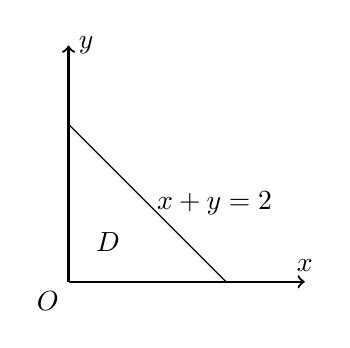
\begin{tikzpicture}
\draw[thick,->] (0,0) -> (3,0)node[above]{\(x\)};
\draw[thick,->] (0,0) -> (0,3)node[right]{\(y\)};
\draw (.5,.5)node{\(D\)};
\draw (0,0)node[below left]{\(O\)};
\draw (0,2)--(2,0)node[midway,right]{\(x+y=2\)};
\end{tikzpicture}
\subcaption{}
\end{subfigure}%
\begin{subfigure}[b]{\subwidth}
\centering
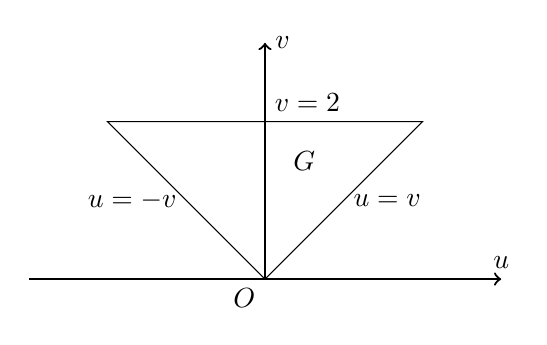
\begin{tikzpicture}
\draw[thick,->] (-3,0) -> (3,0)node[above]{\(u\)};
\draw[thick,->] (0,0) -> (0,3)node[right]{\(v\)};
\draw (.5,1.5)node{\(G\)};
\draw (0,0)node[below left]{\(O\)};
\draw (0,0)--(2,2)node[midway,right]{\(u=v\)}
    --(-2,2)node[midway,above right]{\(v=2\)}
    --(0,0)node[midway,left]{\(u=-v\)};
\end{tikzpicture}
\subcaption{}
\end{subfigure}%
\caption{}
\end{figure}

雅克比式为\[
J = \jacobi{x,y}{u,v}
= \def\arraystretch{1.5} \begin{vmatrix}
-\frac{1}{2} & \frac{1}{2} \\
\frac{1}{2} & \frac{1}{2}
\end{vmatrix}
= - \frac{1}{2}.
\]那么\begin{align*}
\iint_D \exp(\frac{y-x}{y+x}) \dd{x} \dd{y}
&= \iint_G e^{\frac{u}{v}} \abs{-\frac{1}{2}} \dd{u} \dd{v} \\
&= \frac{1}{2} \int_0^2 \dd{v} \int_{-v}^v e^{\frac{u}{v}} \dd{u} \\
&= \frac{1}{2} \int_0^2 \left( e - e^{-1} \right) v \dd{v}
= e - e^{-1}.
\end{align*}
\end{solution}
\end{example}

\begin{example}
计算\(\iint_D \sqrt{1 - \frac{x^2}{a^2} - \frac{y^2}{b^2}} \dd{x} \dd{y}\),%
其中\(D\)是椭圆\(\frac{x^2}{a^2} + \frac{y^2}{b^2} = 1\ (a,b>0)\)所围成的闭区域.
\begin{solution}
作广义极坐标变换\[
\left\{ \begin{array}{l}
x = a \rho \cos\theta, \\
y = b \rho \sin\theta.
\end{array} \right.
\]
在这变换下,与\(D\)对应的闭区域为\(G = \Set{\opair{\rho,\theta} \given 0\leqslant\rho\leqslant1,0\leqslant\theta\leqslant2\pi}\),雅克比式\[
J = \jacobi{x,y}{\rho,\theta} = ab\rho.
\]由于\(J\)仅当\(\rho=0\)时为零,所以换元公式仍成立,从而有\[
\iint_D \sqrt{1 - \frac{x^2}{a^2} - \frac{y^2}{b^2}} \dd{x} \dd{y}
= \iint_G \sqrt{1-\rho^2} ab\rho \dd{\rho} \dd{\theta}
= \frac{2}{3} \pi ab.
\]
\end{solution}
\end{example}

\section{三重积分}
\subsection{三重积分的概念}
定积分及二重积分作为和的极限的概念,可以很自然地推广到三重积分.
\begin{definition}
设\(f(x,y,z)\)是空间有界闭区域\(\Omega\)上的有界函数.将\(\Omega\)任意分成\(n\)个小闭区域\[
\increment v_1,\, \increment v_2,\, \dotsc,\, \increment v_n,
\]其中\(\increment v_i\)表示第\(i\)个小闭区域,
也表示它的体积.在每个\(\increment v_i\)上任取一点\(\opair{\xi_i,\eta_i,\zeta_i}\),
作乘积\(f(\xi_i,\eta_i,\zeta_i) \increment v_i\ (i=1,2,\dotsc,n)\),
并作和\(\sum\limits_{i=1}^n f(\xi_i,\eta_i,\zeta_i) \increment v_i\).
如果当各小闭区域直径中的最大值\(\lambda\)趋于零时这和的极限总存在,
则称此极限为“函数\(f(x,y,z)\)在闭区域\(\Omega\)上的\DefineConcept{三重积分}(triple integral)”,
记作\(\iiint_{\Omega} f(x,y,z) \dd{v}\),即\[
\iiint_{\Omega} f(x,y,z) \dd{v}
= \lim\limits_{\lambda\to0} \sum\limits_{i=1}^n f(\xi_i,\eta_i,\zeta_i) \increment v_i,
\eqno{(1)}
\]其中\(\dd{v}\)叫做\DefineConcept{体积元素}.
\end{definition}

在直角坐标系中,如果用平行于坐标面的平面来划分\(\Omega\),那么除了包含\(\Omega\)的边界点的一些不规则小闭区域外,得到的小闭区域\(\increment v_i\)为长方体.设长方体小闭区域\(\increment v_i\)的边长为\(\increment x_j,\increment y_k,\increment z_l\),则\(\increment v_i = \increment x_j \increment y_k \increment z_l\).因为在直角坐标系中,有时也把体积元素\(\dd{v}\)记作\(\dd{x}\dd{y}\dd{z}\),而把三重积分记作\[
\iiint_{\Omega} f(x,y,z) \dd{x}\dd{y}\dd{z},
\]其中\(\dd{x}\dd{y}\dd{z}\)叫做\DefineConcept{直角坐标系中的体积元素}.

当函数\(f(x,y,z)\)在闭区域\(\Omega\)上连续时,(1)式右端的和的极限必定存在,也就是函数\(f(x,y,z)\)在闭区域\(\Omega\)上的三重积分必定存在.以后我们总假定函数\(f(x,y,z)\)在闭区域\(\Omega\)上是连续的.关于二重积分的一些术语,例如被积函数、积分区域等,也可相应地用到三重积分上.三重积分的性质也与第一节中所叙述的二重积分的性质相类似,这里不再重复了.

如果\(f(x,y,z)\)表示某物体在点\(\opair{x,y,z}\)处的密度,\(\Omega\)是该物体所占有的空间闭区域,\(f(x,y,z)\)在\(\Omega\)上连续,则\(\sum\limits_{i=1}^n f(\xi_i,\eta_i,\zeta_i) \increment v_i\)是该物体的质量\(m\)的近似值,这个和当\(\lambda\to0\)时的极限就是该物体的质量\(m\),所以\[
m = \iiint_{\Omega} f(x,y,z) \dd{v}.
\]

\subsection{三重积分的计算法}
计算三重积分的基本方法是将三重积分化为三次积分来计算.下面按利用不同的坐标来分别讨论将三重积分化为三次积分的方法,且只限于叙述方法.

\subsubsection{利用直角坐标系计算三重积分}
假设平行于\(z\)轴且穿过闭区域\(\Omega\)内部的直线与闭区域\(\Omega\)的边界曲面\(S\)相交不多于两点.把闭区域\(\Omega\)投影到\(xOy\)平面上,得一平面闭区域\(D_{xy}\).以\(D_{xy}\)为边界为准线作母线平行于\(z\)轴的柱面.这柱面与曲面\(S\)的交线从\(S\)中分出的上、下两部分,它们的方程分别为\begin{gather*}
S_1 : z = z_1(x,y), \\
S_2 : z = z_2(x,y),
\end{gather*}其中\(z_1(x,y)\)与\(z_2(x,y)\)都是\(D_{xy}\)上的连续函数,且\(z_1(x,y) \leqslant z_2(x,y)\).
过\(D_{xy}\)内任一点\(\opair{x,y}\)作平行于\(z\)轴的直线,这直线通过曲面\(S_1\)穿入\(\Omega\)内,然后通过曲面\(S_2\)穿出\(\Omega\)外,穿入点与穿出点的竖坐标分别为\(z_1(x,y)\)与\(z_2(x,y)\).

这种情况下,积分区域\(\Omega\)可表示为\[
\Omega = \Set{ \opair{x,y,z} \given z_1(x,y) \leqslant z \leqslant z_2(x,y) \land \opair{x,y} \in D_{xy} }.
\]

先将\(x,y\)看作固定值,将\(f(x,y,z)\)只看做\(z\)的函数,在区间\([z_1(x,y),z_2(x,y)]\)上对\(z\)积分.积分的结果是\(x\)、\(y\)的函数,记作\(F(x,y)\),即\[
F(x,y)=\int_{z_1(x,y)}^{z_2(x,y)} f(x,y,z) \dd{z}.
\]然后计算\(F(x,y)\)在闭区域\(D_{xy}\)上的二重积分\[
\iint_{D_{xy}} F(x,y) \dd{\sigma}
=\iint_{D_{xy}} \left[
 \int_{z_1(x,y)}^{z_2(x,y)} f(x,y,z) \dd{z}
\right] \dd{\sigma}.
\]假如闭区域\[
D_{xy} = \Set{ \opair{x,y} \given y_1(x) \leqslant y \leqslant y_2(x) \land a \leqslant x \leqslant b },
\]把这个二重积分化为二次积分,于是得到三重积分的计算公式\[
\iiint_{\Omega} f(x,y,z) \dd{v}
= \int_a^b  \dd{x} \int_{y_1(x)}^{y_2(x)} \dd{y} \int_{z_1(x,y)}^{z_2(x,y)} f(x,y,z) \dd{z}.
\eqno{(2)}
\]公式(2)把三重积分化为先对\(z\)、再对\(y\)、最后对\(x\)的三次积分.

如果平行于\(x\)轴或\(y\)轴且穿过闭区域\(\Omega\)内部的直线与\(\Omega\)的边界曲面\(S\)相交不多于两点,也可把闭区域\(\Omega\)投影到\(yOz\)面上或\(xOz\)面上,这样便可把三重积分化为按其他顺序的三次积分.如果平行于坐标轴且穿过闭区域\(\Omega\)内部的直线与边界曲面\(S\)的交点多于两个,也可像处理二重积分那样,把\(\Omega\)分成若干部分,使\(\Omega\)上的三重积分化为各部分闭区域上的三重积分的和.

\begin{example}
计算三重积分\(\iiint_{\Omega} x \dd{x}\dd{y}\dd{z}\),其中\(\Omega\)是三个坐标面及平面\(x+2y+z=1\)所围成的闭区域.
\begin{solution}
将\(\Omega\)投影到\(xOy\)面上,得投影区域\(D_{xy}\)为三角形闭区域\[
D_{xy} = \Set{ \opair{x,y} \given 0 \leqslant \frac{1-x}{2}, 0 \leqslant x \leqslant 1 }.
\]

在\(D_{xy}\)内任取一点\(\opair{x,y}\),过此点作平行于\(z\)轴的直线,该直线通过平面\(z = 0\)穿入\(\Omega\)内,然后通过平面\(z = 1 - x - 2y\)穿出\(\Omega\)外.于是由公式(2)得\begin{align*}
\iiint_{\Omega} x \dd{x}\dd{y}\dd{z}
&= \int_0^1 \dd{x} \int_0^{(1-x)/2} \dd{y} \int_0^{1-x-2y} x \dd{z} \\
&= \int_0^1 x \dd{x} \int_0^{(1-x)/2} (1-x-2y) \dd{y} \\
&= \frac{1}{4} \int_0^1 (x - 2x^2 + x^3) \dd{x}
= \frac{1}{48}.
\end{align*}
\end{solution}
\end{example}

有时,我们计算一个三重积分也可以化为先计算一个二重积分、再计算一个定积分,即有下述计算公式.

设空间闭区域\[
\Omega = \Set{ \opair{x,y,z} \given c_1 \leqslant z \leqslant c_2 \land \opair{x,y} \in D_z },
\]其中\(D_z\)是竖坐标为\(z\)的平面截空间闭区域\(\Omega\)所得到的一个平面闭区域,则有\[
\iiint_{\Omega} f(x,y,z) \dd{v}
=\int_{c_1}^{c_2} \dd{z} \iint_{D_{z}} f(x,y,z) \dd{x}\dd{y}.
\eqno{(3)}
\]

\begin{example}
计算三重积分\(\iiint_{\Omega} z^2 \dd{x}\dd{y}\dd{z}\),其中\(\Omega\)是由椭球面\(\frac{x^2}{a^2}+\frac{y^2}{b^2}+\frac{z^2}{c^2}=1\)所围成的空间闭区域.
\begin{solution}
空间闭区域\(\Omega\)可表示为\[
\Set*{ \opair{x,y,z} \given \frac{x^2}{a^2}+\frac{y^2}{b^2}\leqslant1-\frac{z^2}{c^2}, -c \leqslant z \leqslant c }.
\]由公式(3)得\[
\iiint_{\Omega} z^2 \dd{x}\dd{y}\dd{z}
= \int_{-c}^c z^2 \dd{z} \iint_{D_z} \dd{x}\dd{y} = \pi ab \int_{-c}^c \left(1-\frac{z^2}{c^2}\right) z^2 \dd{z} = \frac{4}{15}\pi abc^3.
\]
\end{solution}
\end{example}

\subsubsection{利用柱面坐标系计算三重积分}
利用以下关系\[
\left\{ \begin{array}{l}
x = \rho\cos\theta \\
y = \rho\sin\theta \\
z = z \\
\end{array} \right.
\]替换三重积分\(\iiint_{\Omega}{f(x,y,z)\dd{x}\dd{y}\dd{z}}\)中的积分变量,即有\[
\iiint_{\Omega}{f(x,y,z)\dd{x}\dd{y}\dd{z}}
= \iiint_{\Omega}{f(\rho \cos\theta,\rho \sin\theta,z) \rho \dd{\rho} \dd{\theta} \dd{z}},
\]其中,\(\dd{v} = \rho \dd{\rho} \dd{\theta} \dd{z}\)称为\DefineConcept{柱面坐标系中的体积元素}.

\subsubsection{利用球面坐标系计算三重积分}
利用以下关系\[
\left\{ \begin{array}{l}
x = r \sin\varphi \cos\theta, \\
y = r \sin\varphi \sin\theta, \\
z = r \cos\varphi
\end{array} \right.
\]替换三重积分\(\iiint_{\Omega}{f(x,y,z)\dd{x}\dd{y}\dd{z}}\)中的积分变量,即有\[
\iiint_{\Omega}{f(x,y,z)\dd{x}\dd{y}\dd{z}}
= \iiint_{\Omega}{f(r \sin\varphi \cos\theta,r \sin\varphi \sin\theta,r \cos\varphi) r^2 \sin\varphi \dd{r} \dd{\varphi} \dd{\theta}},
\]其中,\(\dd{v} = r^2 \sin\varphi \dd{r} \dd{\varphi} \dd{\theta}\)称为\DefineConcept{球面坐标系中的体积元素}.

\begin{example}
证明:半径为\(R\)的球的体积为\(V = \frac{4}{3} \pi R^3\).
\begin{proof}
以球心为原点建立球面坐标系,得球的方程为\[
\Omega: r \leqslant R.
\]那么球的体积为\begin{align*}
V &= \iiint_{\Omega} r^2 \sin\varphi \dd{r} \dd{\varphi} \dd{\theta} \\
&= \int_0^R r^2 \dd{r} \int_0^{\pi} \sin\varphi \dd{\varphi} \int_0^{2\pi} \dd{\theta} \\
&= \frac{1}{3} R^3 \cdot 2 \cdot 2\pi
= \frac{4}{3} \pi R^3.
\qedhere
\end{align*}
\end{proof}
\end{example}

\section{扩展:多重积分的一般性理论}
\subsection{重积分化为累次积分}
\begin{theorem}[富比尼定理]
设区域\(X\subseteq\mathbb{R}^m, Y\subseteq\mathbb{R}^n\).
如果函数\(f\colon X \times Y \to \mathbb{R}\)在\(X \times Y\)上可积,则\(f\)的重积分与累次积分同时存在且彼此相等,即\[
\int_{X \times Y} f(x,y) \dd{x}\dd{y}
= \int_X \dd{x} \int_Y f(x,y) \dd{y}
= \int_Y \dd{y} \int_X f(x,y) \dd{x}.
\]
\end{theorem}

\begin{corollary}
如果函数\(f\in\mathcal{R}(X \times Y)\),则(在勒贝格意义下)%
对于几乎所有的值\(x \in X\),积分\(\int_Y f(x,y) \dd{y}\)存在;%
对于几乎所有的值\(y \in Y\),积分\(\int_X f(x,y) \dd{x}\)存在.
\end{corollary}

\begin{corollary}
\newcommand\intx[2][]{\int_{a_{#2}}^{b_{#2}} #1 \dd{x_{#2}}}%
如果区间\(I \subseteq \mathbb{R}^n\)是闭区域\(I_i = [a_i,b_i]\ (i=1,2,\dotsc,n)\)的直积,则\[
\int_I f(x) \dd{x}
= \intx{n} \intx{n-1} \dotso \intx[f(\AutoTuple{x}{n})]{1}.
\]
\end{corollary}

\subsection{重积分中的变量代换}
利用雅克比式,可以把二重积分的换元法推广到多元函数上.
\begin{theorem}
若连续可微函数\[
\mat{y} = f(\mat{x})
\quad(\mat{x},\mat{y}\in\mathbb{R}^n)
\]把\(O x_1 x_2 \dotso x_n\)空间内的有界闭区域\(\Omega\)单值地映射成\(O' y_1 y_2 \dotso y_n\)空间内的有界闭区域\(\Omega'\),并且在闭区域\(\Omega'\)内雅克比行列式\[
J = \det\mat{J}
= \jacobi{f_1,f_2,\dotsc,f_n}{\AutoTuple{x}{n}}
= {
\def\arraystretch{1.5}
\begin{vmatrix}
\pdv{f_1}{x_1} & \pdv{f_1}{x_2} & \dots & \pdv{f_1}{x_n} \\
\pdv{f_2}{x_1} & \pdv{f_2}{x_2} & \dots & \pdv{f_2}{x_n} \\
\vdots & \vdots & \ddots & \vdots \\
\pdv{f_n}{x_1} & \pdv{f_n}{x_2} & \dots & \pdv{f_n}{x_n} \\
\end{vmatrix}
}
\neq 0,
\]则有如下的积分换元公式\begin{equation}
\begin{split}
&\idotsint\limits_{\Omega} F(\AutoTuple{y}{n}) \dd{y_1}\dd{y_2}\dotsm\dd{y_n} \\
&\hspace{20pt}= \idotsint\limits_{\Omega} F(\AutoTuple{x}{n}) \abs{J} \dd{x_1}\dd{x_2}\dotsm\dd{x_n}.
\end{split}
\end{equation}
\end{theorem}
利用上述积分换元公式可以将复杂的被积函数化简,也可以将复杂的积分区域化为更具对称性的积分区域.


\section{重积分的应用}
\subsection{利用重积分的定义计算极限}
\begin{example}
用二重积分的定义计算极限\[
\lim\limits_{n\to\infty} \sum\limits_{i=1}^n \sum\limits_{j=1}^n \frac{n}{(n+i)(n^2+j^2)}.
\]
\begin{solution}
首先观察极限
\begin{align*}
&\hspace{-20pt}
\lim\limits_{n\to\infty} \sum\limits_{i=1}^n \sum\limits_{j=1}^n \frac{n}{(n+i)(n^2+j^2)} \\
&= \lim\limits_{n\to\infty} \sum\limits_{i=1}^n \sum\limits_{j=1}^n \frac{1}{n^2} \frac{n^3}{(n+i)(n^2+j^2)} \\
&= \lim\limits_{n\to\infty} \sum\limits_{i=1}^n \sum\limits_{j=1}^n \frac{1}{n^2} \left[\left(1+\frac{i}{n}\right)\left(1+\frac{j^2}{n^2}\right)\right]^{-1},
\end{align*}
考虑当\(i=j=1\)时,\(\frac{i}{n},\frac{j}{n}\to0\ (n\to\infty)\);
当\(i=j=n\)时,\(\frac{i}{n}=\frac{j}{n}=1\);
那么可以将所求极限视作函数\(\frac{1}{1+x}\cdot\frac{1}{1+y^2}\)在区域\([0,1]\times[0,1]\)上的积分\[
\int_0^1 \dd{x} \int_0^1 \frac{1}{(1+x)(1+y^2)} \dd{y}
= \int_0^1 \frac{1}{1+x} \dd{x} \int_0^1 \frac{1}{1+y^2} \dd{y}.
\]
\end{solution}
\end{example}

\subsection{曲面的面积}
设两平面\(\Pi_1\)、\(\Pi_2\)的夹角为\(\theta\ (0<\theta<\pi/2)\)(如\cref{figure:重积分.平面区域的投影}),%
\(\Pi_1\)上的闭区域\(D\)在\(\Pi_2\)上的投影区域为\(D_0\),%
则\(D\)的面积\(A\)与\(D_0\)的面积\(\sigma\)满足\[
A = \frac{\sigma}{\cos\theta}.
\]
事实上,先假定\(D\)是矩形闭区域,且其一边平行于平面\(\Pi_1\)、\(\Pi_2\)的交线\(l\),%
两条边的边长分别为\(a\)、\(b\),则\(D_0\)也是矩形闭区域,%
且边长分别为\(a\)、\(b \cos\theta\),从而\[
\sigma = ab\cos\theta = A \cos\theta.
\]

\begin{figure}[ht]
\centering
\begin{tikzpicture}[scale=2]
\draw[name path=upper](0,0)--++(1,-1)node[midway,below left]{\(l\)}coordinate(p1)
	--++(2,2)coordinate(p2)
	--++(-1,1)node[below]{\(\Pi_1\)}
	--++(-2,-2);
\path[name path=horizon](1,0)--++(2,0);
\draw[name intersections={of=upper and horizon},dashed]
	(intersection-1)--(0,0);
\draw(p1)--++(3,0)coordinate(p3)
	--++(-1,1)node[below]{\(\Pi_2\)}
	--(intersection-1);
\draw pic["\(\theta\)",draw=orange,-,angle eccentricity=2,angle radius=0.3cm]{angle=p3--p1--p2};
\draw(1.6,.9)coordinate(A)
	--++(.3,-.3)coordinate(B)node[midway,below left]{\(a\)}
	--++(.2,.2)coordinate(C)node[midway,below right]{\(b\)}
	--++(-.3,.3)coordinate(D)
	--++(-.2,-.2);
\begin{scope}[dashed]
\draw(A)--++(0,-1.4)coordinate(A1);
\draw(B)--++(0,-1.4)coordinate(B1);
\draw(C)--++(0,-1.4-.2)coordinate(C1);
\draw(D)--++(0,-1.4-.2)coordinate(D1);
\end{scope}
\draw(A1)--(B1)node[midway,below left]{\(a\)}--(C1)node[midway,below]{\(b \cos\theta\)}--(D1)--(A1);
\end{tikzpicture}
\caption{平面区域的投影}
\label{figure:重积分.平面区域的投影}
\end{figure}

\begin{theorem}
设曲面\(S\)由方程\[
z=f(x,y)
\]给出,\(D_{xy}\)为曲面\(S\)在\(xOy\)面上的投影区域,%
函数\(f(x,y)\)在\(D_{xy}\)上具有连续偏导数\(f'_x(x,y)\)和\(f'_y(x,y)\).
那么曲面\(S\)面积元素\(\dd{A}\)为\[
\dd{A} = \sqrt{1 + [f'_x(x,y)]^2 + [f'_y(x,y)]^2} \dd{\sigma}.
\]

曲面\(S\)的面积为\begin{align}
A &= \iint_{D_{xy}} \sqrt{1 + [f'_x(x,y)]^2 + [f'_y(x,y)]^2} \dd{\sigma} \nonumber \\
&= \iint_{D_{xy}} \sqrt{1 + \left(\pdv{z}{x}\right)^2 + \left(\pdv{z}{y}\right)^2} \dd{x}\dd{y}.
\end{align}
\end{theorem}

设曲面的方程为\(x=g(y,z)\)或\(y=h(z,x)\),%
可分别把曲面投影到\(yOz\)面上(投影区域记作\(D_{yz}\))或\(zOx\)面上(投影区域记作\(D_{zx}\)),%
类似地可得\begin{equation}
A = \iint_{D_{yz}} \sqrt{1 + \left(\pdv{x}{y}\right)^2 + \left(\pdv{x}{z}\right)^2} \dd{y}\dd{z},
\end{equation}或\begin{equation}
A = \iint_{D_{zx}} \sqrt{1 + \left(\pdv{y}{z}\right)^2 + \left(\pdv{y}{x}\right)^2} \dd{z}\dd{x}.
\end{equation}

\begin{example}
求半径为\(R\)的球的表面积.
\begin{solution}
\def\z{\sqrt{R^2-x^2-y^2}}
取上半球面方程为\(z = \z\),则它在\(xOy\)面上的投影区域为\[
D = \Set{\opair{x,y} \given x^2+y^2 \leqslant R^2}.
\]由\[
\pdv{z}{x} = \frac{-x}{\z},
\qquad
\pdv{z}{y} = \frac{-y}{\z},
\]得\[
\sqrt{1 + \left(\pdv{y}{z}\right)^2 + \left(\pdv{y}{x}\right)^2}
= \frac{R}{\z}.
\]因为这函数在闭区域\(D\)上无界,我们不能直接应用曲面面积公式,所以先取区域\[
D_1 = \Set{\opair{x,y} \given x^2+y^2 \leqslant r^2}
\quad(0<r<R)
\]为积分区域,算出相应于\(D_1\)上的球面面积\[
A_1 = \iint_{D_1} \frac{R}{\z} \dd{x}\dd{y}
\]后,令\(r \to R\)取\(A_1\)的极限就得半球面的面积.

\def\zz{\sqrt{R^2-\rho^2}}
利用极坐标,得\[
A_1 = \iint_{D_1} \frac{R}{\zz} \rho\dd{\rho}\dd{\theta}
= R \int_0^{2\pi} \dd{\theta} \int_0^r \frac{\rho \dd{\rho}}{\zz}
= 2\pi R(R-\sqrt{R^2-r^2}),
\]
\def\l{\lim\limits_{r \to R}}
于是\begin{equation}
A = \l A_1
= \l 2\pi R(R-\sqrt{R^2-r^2})
= 2\pi R^2.
\end{equation}
\end{solution}
\end{example}

\begin{theorem}[利用曲面的参数方程求曲面的面积]
设曲面\(S\)由参数方程\[
\left\{ \begin{array}{l}
x = x(u,v), \\
y = y(u,v), \\
z = z(u,v) \\
\end{array} \right.
\quad
\opair{u,v} \in D
\]给出,其中\(D\)是一个平面有界闭区域,又\(x(u,v), y(u,v), z(u,v)\)在\(D\)上具有连续的一阶偏导数,且\[
\jacobi{x,y}{u,v}, \qquad
\jacobi{y,z}{u,v}, \qquad
\jacobi{z,x}{u,v}
\]不全为零,则曲面\(S\)的面积为
\begin{equation}\label{equation:重积分.曲面的面积计算公式}
A = \iint_D \sqrt{E G - F^2} \dd{u}\dd{v},
\end{equation}其中\begin{align*}
E &= (x'_u)^2 + (y'_u)^2 + (z'_u)^2, \\
F &= x'_u \cdot x'_v + y'_u \cdot y'_v + z'_u \cdot z'_v, \\
G &= (x'_v)^2 + (y'_v)^2 + (z'_v)^2.
\end{align*}
\rm
上述\(E\)、\(F\)和\(G\)又称为曲面的\DefineConcept{高斯系数}.
\end{theorem}
\begingroup
\def\J{\mat{J}}%
\cref{equation:重积分.曲面的面积计算公式} 也可记作\[
A = \iint_D \sqrt{\det(\J^T \J)} \dd{u}\dd{v},
\]其中雅克比矩阵\[
\J = \begin{bmatrix}
x'_u & x'_v \\
y'_u & y'_v \\
z'_u & z'_v
\end{bmatrix}.
\]
\endgroup

\subsection{物体的质心}
\begin{theorem}
设物体占有空间有界闭区域\(\Omega\),其在点\(\opair{x,y,z}\)处的密度为\[
\rho=\rho(x,y,z)
\](假定\(\rho(x,y,z)\)在\(\Omega\)上连续),则其质心坐标为\begin{equation}
\opair*{
\frac{1}{M} \iiint_{\Omega} x \rho \dd{v},
\frac{1}{M} \iiint_{\Omega} y \rho \dd{v},
\frac{1}{M} \iiint_{\Omega} z \rho \dd{v}
}
\end{equation}其中\(M = \iiint_{\Omega} \rho \dd{v}\).
\end{theorem}

\subsection{物体的转动惯量}
\begin{theorem}
设物体占有空间有界闭区域\(\Omega\),其在点\(\opair{x,y,z}\)处的密度为\[
\rho=\rho(x,y,z)
\](假定\(\rho(x,y,z)\)在\(\Omega\)上连续),则其相对于\(x\)、\(y\)、\(z\)轴的转动惯量为\begin{align}
I_x &= \iiint_{\Omega} (y^2+z^2) \rho(x,y,z) \dd{v}, \\
I_y &= \iiint_{\Omega} (z^2+x^2) \rho(x,y,z) \dd{v}, \\
I_z &= \iiint_{\Omega} (x^2+y^2) \rho(x,y,z) \dd{v}.
\end{align}
\end{theorem}

\subsection{引力}
\begin{theorem}
设引力常量为\(G\),物体占有空间有界闭区域\(\Omega\),它在点\(\opair{x,y,z}\)处的密度为\[
\rho=\rho(x,y,z),
\]并假定\(\rho(x,y,z)\)在\(\Omega\)上连续,则其对物体外一点\(P_0\opair{x_0,y_0,z_0}\)的引力为\begin{equation}
\mat{F}
= \opair*{
G \cdot \iiint_{\Omega} \frac{\rho (x-x_0)}{r^3} \dd{v},
G \cdot \iiint_{\Omega} \frac{\rho (y-y_0)}{r^3} \dd{v},
G \cdot \iiint_{\Omega} \frac{\rho (z-z_0)}{r^3} \dd{v}
}.
\end{equation}
\end{theorem}

\section{含参变量的积分}
\subsection{含参变量积分的概念与性质}
设\(f(x,y)\)是矩形(闭区域)\(R = [a,b]\times[c,d]\)上的连续函数.
在\([a,b]\)上任意取定\(x\)的一个值,于是\(f(x,y)\)是变量\(y\)在\([c,d]\)上的一个一元连续函数,从而积分\[
\int_c^d f(x,y) \dd{y}
\]存在,这个积分的值依赖于取定的\(x\)的值.
当\(x\)的值改变时,一般来说这个积分的值也跟着改变.
这个积分确定一个定义在\([a,b]\)上的关于\(x\)的函数,若将其记为\(\varphi(x)\),则有\[
\varphi(x) = \int_c^d f(x,y) \dd{y}
\quad(a \leqslant x \leqslant b).
\]这里变量\(x\)在积分过程中看作是一个常量,通常称其为\DefineConcept{参变量},因此上式右端是一个含参变量\(x\)的积分,这个积分确定关于\(x\)的一个函数\(\varphi(x)\).
下面讨论关于\(\varphi(x)\)的一些性质.

\begin{theorem}
如果函数\(f(x,y)\)在矩形\(R=[a,b]\times[c,d]\)上连续,%
那么函数\[
\varphi(x) = \int_c^d{f(x,y)\dd{y}}, \quad a \leqslant x \leqslant b
\]在\([a,b]\)上也连续.
\end{theorem}

\begin{theorem}
如果函数\(f(x,y)\)在矩形\(R=[a,b]\times[c,d]\)上连续,则\[
\int_a^b\left[\int_c^d f(x,y) \dd{y}\right] \dd{x}
=\int_c^d\left[\int_a^b f(x,y) \dd{x}\right] \dd{y}.
\]
\end{theorem}
上式也可写成\[
\int_a^b \dd{x} \int_c^d f(x,y) \dd{y}
=\int_c^d \dd{y} \int_a^b f(x,y) \dd{x}.
\]

\begin{theorem}
如果函数\(f(x,y)\)及其偏导数\(f'_x(x,y)\)都在矩形\(R=[a,b]\times[c,d]\)上连续,那么函数\[
\varphi(x) = \int_c^d f(x,y) \dd{y}
\quad(a \leqslant x \leqslant b)
\]在\([a,b]\)上可微,并且\[
\varphi'(x) = \dv{x} \int_c^d f(x,y) \dd{y}
= \int_c^d f'_x(x,y) \dd{y}.
\]
\end{theorem}

\begin{theorem}
如果函数\(f(x,y)\)在矩形\(R=[a,b]\times[c,d]\)上连续,%
函数\(\alpha(x)\)与\(\beta(x)\)在区间\([a,b]\)上连续,且\[
x \in [a,b] \implies \alpha(x),\beta(x) \in [c,d],
\]则函数\[
\Phi(x) = \int_{\alpha(x)}^{\beta(x)} f(x,y)\dd{y}
\quad(a \leqslant x \leqslant b)
\]在\([a,b]\)上也连续.
\end{theorem}

\begin{theorem}
如果函数\(f(x,y)\)及其偏导数\(f'_x(x,y)\)都在矩形\(R=[a,b]\times[c,d]\)上连续,%
函数\(\alpha(x)\)与\(\beta(x)\)在区间\([a,b]\)上可微,且\[
x \in [a,b] \implies \alpha(x),\beta(x) \in [c,d],
\]则函数\[
\Phi(x) = \int_{\alpha(x)}^{\beta(x)} f(x,y)\dd{y}
\quad(a \leqslant x \leqslant b)
\]在\([a,b]\)上也可微,且\begin{align*}
\Phi'(x) &= \dv{x} \int_{\alpha(x)}^{\beta(x)} f(x,y) \dd{y} \\
&= \int_{\alpha(x)}^{\beta(x)} f'_x(x,y) \dd{y}
	+ f[x,\beta(x)] \cdot \beta'(x)
	- f[x,\alpha(x)] \cdot \alpha'(x).
\end{align*}
\end{theorem}
上式也被称为\DefineConcept{莱布尼茨公式}.

\begin{example}
设\(F(x) = \int_x^{x^2} \frac{\sin xy}{y} \dd{y}\),求\(F'(x)\).
\begin{solution}
应用莱布尼茨公式,得\begin{align*}
F'(x) &= \int_x^{x^2} \cos xy \dd{y}
+ \frac{\sin x^3}{x^2} \cdot 2x
- \frac{\sin x^2}{x} \cdot 1 \\
&= \left[ \frac{\sin xy}{x} \right]_x^{x^2}
+ \frac{2 \sin x^3}{x}
- \frac{\sin x^2}{x}
= \frac{3 \sin x^3 - 2 \sin x^2}{x}.
\end{align*}
\end{solution}
\end{example}

\begin{example}
求\(I = \int_0^1 \frac{x^b-x^a}{\ln x} \dd{x}\ (0<a<b)\).
\begin{solution}
因为\[
\int_a^b x^y \dd{y}
= \left[ \frac{x^y}{\ln x} \right]_a^b
= \frac{x^b - x^a}{\ln x},
\]所以\[
I = \int_0^1 \dd{x} \int_a^b x^y \dd{y}.
\]这里函数\(f(x,y) = x^y\)在矩形\(R=[0,1]\times[a,b]\)上连续,那么只要交换积分次序,就有\[
I = \int_a^b \dd{y} \int_0^1 x^y \dd{x}
= \int_a^b \left[\frac{x^{y+1}}{y+1}\right]_0^1 \dd{y}
= \int_a^b \frac{1}{y+1} \dd{y}
= \ln\frac{b+1}{a+1}.
\]
\end{solution}
\end{example}

\begin{example}
计算定积分\(I = \int_0^1 \frac{\ln(1+x)}{1+x^2} \dd{x}\).
\begin{solution}
考虑含参变量\(\alpha\)的积分所确定的函数\[
\varphi(\alpha) = \int_0^1 \frac{\ln(1+\alpha x)}{1+x^2} \dd{x}.
\]显然,\(\varphi(0) = 0\),\(\varphi(1) = I\).
对\(\varphi(\alpha)\)求导得\[
\varphi'(\alpha)
= \int_0^1 \frac{x}{(1+\alpha x)(1+x^2)} \dd{x}.
\]把被积函数分解为部分分式,得到\[
\frac{x}{(1+\alpha x)(1+x^2)}
= \frac{1}{1+\alpha^2} \left[
\frac{-\alpha}{1+\alpha x}
+ \frac{x}{1+x^2}
+ \frac{\alpha}{1+x^2}
\right].
\]于是\begin{align*}
\varphi'(\alpha)
&= \frac{1}{1+\alpha^2} \left[
\int_0^1 \frac{-\alpha \dd{x}}{1+\alpha x}
+ \int_0^1 \frac{x \dd{x}}{1+x^2}
+ \int_0^1 \frac{\alpha \dd{x}}{1+x^2}
\right] \\
&= \frac{1}{1+\alpha^2} \left[
-\ln(1+\alpha)
+ \frac{1}{2} \ln2
+ \alpha \cdot \frac{\pi}{4}
\right],
\end{align*}
上式在\([0,1]\)上对\(\alpha\)积分,得到\begin{align*}
I &= \varphi(1)-\varphi(0)
= \int_0^1 \varphi'(\alpha) \dd{\alpha} \\
&= - \int_0^1 \frac{\ln(1+\alpha)}{1+\alpha^2} \dd{\alpha}
+ \frac{1}{2} \ln2 \int_0^1 \frac{\dd{\alpha}}{1+\alpha^2}
+ \frac{\pi}{4} \int_0^1 \frac{\alpha}{1+\alpha^2} \dd{\alpha} \\
&= -I + \frac{\ln2}{2} \cdot \frac{\pi}{4} + \frac{\pi}{4}\cdot\frac{\ln2}{2}
= -I + \frac{\pi}{4} \ln2,
\end{align*}
解得\(I = \frac{\pi}{8} \ln2\).
\end{solution}
\end{example}

\begin{example}
求函数\(f(x) = \int_1^{x^2} (x^2-t) e^{-t^2} \dd{t}\)的单调区间与极值.
\begin{solution}
求导得\[
\dv{f}{x}
= \int_1^{x^2} \pdv{x} (x^2-t) e^{-t^2} \dd{t}
= 2x \int_1^{x^2} e^{-t^2} \dd{t}.
\]
因为\(e^{-t^2}>0\ (-\infty<t<+\infty)\),所以根据\cref{theorem:定积分.定积分性质5},当\(x^2>1\)时,有\[
\int_1^{x^2} e^{-t^2} \dd{t} > 0;
\]当\(x^2 \leqslant 1\)时,有\[
\int_1^{x^2} e^{-t^2} \dd{t} \leqslant 0.
\]那么\begin{center}
\begin{tabular}{c|*7c}
\hline
\(x\) & \((-\infty,-1)\) & \(-1\) & \((-1,0)\) & \(0\) & \((0,1)\) & \(1\) & \((1,+\infty)\) \\ \hline
\(f'(x)\) & \(-\) & \(0\) & \(+\) & \(0\) & \(-\) & \(0\) & \(+\) \\
\(f(x)\) & \(\searrow\) & \(0\) & \(\nearrow\) & \((1-e^{-1})/2\) & \(\searrow\) & \(0\) & \(\nearrow\) \\
\hline
\end{tabular}
\end{center}
也就是说,函数\(f\)在区间\((-\infty,-1)\cup(0,1)\)上单调减少,在区间\((-1,0)\cup(1,+\infty)\)上单调增加,在点\(\pm1\)处取得极小值\(0\),在点\(0\)处取得极大值\(\frac{1-e^{-1}}{2}\).
\end{solution}
\end{example}
本例若利用\cref{theorem:定积分.定积分性质1} 将\[
\int_1^{x^2} (x^2-t) e^{-t^2} \dd{t}
\]拆开成\[
x^2 \int_1^{x^2} e^{-t^2} \dd{t}
\quad\text{和}\quad
\int_1^{x^2} t e^{-t^2} \dd{t}
\]两个部分,再分别对\(x\)求导,也可以求出\(\dv{f}{x}\).

\begin{example}%《高等数学(第六版 下册)》习题10-5 1.(1)
\def\l{\lim\limits_{x\to0}}%
计算极限\(\l \int_x^{x+1} \frac{\dd{y}}{1+x^2+y^2}\).
\begin{solution}
记\[
f(t) = \int_x^{x+t} \frac{\dd{y}}{1+x^2+y^2},
\]求导得\begin{align*}
f'(t)
&= \int_x^{x+t} \pdv{t}(\frac{1}{1+x^2+y^2}) \dd{y}
+ \frac{1}{1+x^2+(x+t)^2} \cdot 1
- \frac{1}{1+x^2+x^2} \cdot 0 \\
&= \frac{1}{1+x^2+(x+t)^2}.
\end{align*}
因为\(f(0) = 0\),所以
\begin{align*}
&\hspace{-20pt}
\l \int_x^{x+1} \frac{\dd{y}}{1+x^2+y^2} \\
&= f(1) - f(0)
= \int_0^1 f'(t) \dd{t} \\
&= \int_0^1 \frac{\dd{t}}{1+x^2+(x+t)^2} \\
&= \frac{1}{\sqrt{1+x^2}} \int_0^1 \left[1+\frac{(x+t)^2}{1+x^2}\right]^{-1} \dd(\frac{x+t}{\sqrt{1+x^2}}) \\
&= \frac{1}{\sqrt{1+x^2}} \left(\arctan\frac{x+t}{\sqrt{1+x^2}}\right)_0^1 \\
&= \frac{1}{\sqrt{1+x^2}} \left(
\arctan\frac{x+1}{\sqrt{1+x^2}}
- \arctan\frac{x}{\sqrt{1+x^2}}
\right).
\end{align*}
因此\[
\l \int_x^{x+1} \frac{\dd{y}}{1+x^2+y^2}
= \l f(1)
= \l \frac{1}{\sqrt{1+x^2}} \left(
\arctan\frac{x+1}{\sqrt{1+x^2}}
- \arctan\frac{x}{\sqrt{1+x^2}}
\right)
= \frac{\pi}{4}.
\]
\end{solution}
\end{example}

\begin{example}%《高等数学(第六版 下册)》习题10-5 1.(2)
\def\l{\lim\limits_{x\to0}}%
计算极限\(\l \int_{-1}^1 \sqrt{x^2+y^2} \dd{y}\).
\begin{solution}
设\[
f(t)
=\frac{1}{2} \int_{-t}^t \sqrt{x^2+y^2} \dd{y}
=\int_0^t \sqrt{x^2+y^2} \dd{y},
\]
求导得\[
f'(t)
= \int_0^t \pdv{t} \sqrt{x^2+y^2} \dd{y}
	+ \sqrt{x^2+t^2} \cdot 1
= \sqrt{x^2+t^2}.
\]又因为\(f(0) = 0\),所以\begin{align*}
\frac{1}{2} \int_{-1}^1 \sqrt{x^2+y^2} \dd{t}
&=f(1) - f(0)
= \int_0^1 f'(t) \dd{t}
= \int_0^1 \sqrt{x^2+t^2} \dd{t} \\
&= \left[
\frac{t}{2} \sqrt{x^2+t^2} + \frac{x^2}{2} \ln(t+\sqrt{x^2+t^2})
\right]_0^1 \\
&= \frac{1}{2} \sqrt{x^2+1} + \frac{x^2}{2} \left[ \ln(1+\sqrt{x^2+1}) - \ln\abs{x} \right]
\end{align*}
从而\[
\l \int_{-1}^1 \sqrt{x^2+y^2} \dd{y}
= \l \left[
\sqrt{x^2+1}
+ x^2 \ln(1+\sqrt{x^2+1}) - x^2 \ln\abs{x}
\right]
= 1.
\]
\end{solution}
\end{example}

之前我们讲到,在计算反常积分时,%
可以直接利用反常积分的定义%
以及牛顿-莱布尼茨公式.
除此以外,我们还可以从含参变量积分的思路处理复杂的反常积分问题.

\begin{example}
证明反常积分\[
I = \int_0^{+\infty} \frac{\sin x}{x} \dd{x}
\]收敛,并计算它的值.
\begin{proof}
令\(I(a) = \int_0^{+\infty} \frac{\sin x}{x} e^{-ax} \dd{x}\ (a>0)\),于是\(I(0) = I\).
求导得\[
I'(a) = \dv{a} I(a) = \int_0^{+\infty} \frac{\sin x}{x} e^{-ax} (-x) \dd{x}
= - \int_0^{+\infty} e^{-ax} \sin x \dd{x}
= - \frac{1}{a^2+1},
\]再积分得\[
I(a) = -\arctan a + C,
\]其中\(C\)是待定常数.
令\(a\to+\infty\),得\(\arctan a\to\frac{\pi}{2}\),\(\int_0^{+\infty} \frac{\sin x}{x} e^{-ax} \dd{x} \to 0\),所以\(C = \frac{\pi}{2}\).
因此\(I = I(0) = \frac{\pi}{2}\).
\end{proof}
\end{example}
上述反常积分又称为狄利克雷积分,利用留数定理也可以求出它的值.
